\documentclass[11pt,onside]{report}
\usepackage{a4}
\usepackage[a4paper,inner=1.5cm,outer=1.5cm,tmargin=3cm, bmargin=3cm,headsep=1.0cm,bindingoffset=0cm,headheight=14pt]{geometry}
\usepackage[onehalfspacing]{setspace}
\usepackage[utf8]{inputenc}
\usepackage[american]{babel}
\usepackage{fancyhdr}
\pagestyle{fancy}
\fancyhead[RO,LE]{\thepage}
\fancyfoot[C]{\vspace{3pt} \thepage}



\usepackage{multirow}
\usepackage[bf,format=plain]{caption}
\usepackage{xcolor}
\usepackage{graphicx}
\usepackage{wallpaper}
\usepackage{wrapfig}
\usepackage{subfig}
\captionsetup[subfloat]{labelfont={footnotesize,rm,md,up}}
\usepackage{float}
\usepackage{longtable}
\usepackage{booktabs}
\usepackage{enumitem}
\usepackage{placeins}

\usepackage{latexsym,exscale,amssymb,amsmath,amsfonts,amstext,amsbsy,esint}
\usepackage[thinspace,thickqspace,squaren]{SIunits}

\usepackage[babel]{csquotes}


\usepackage[framed]{matlab-prettifier}


\usepackage[
bookmarks=true,
allcolors=black,
allbordercolors=black,
colorlinks=true,
linkcolor=black,
urlcolor=blue,
pdfauthor={Jan Thiart, Simon Christoph Stein, Jan Christoph Thiele},
pdftitle={TrackNTrace Lifetime Edition - Manual},
pdfsubject={Manual},
pdfcreator={Jan Christoph Thiele},
pdfkeywords={}]
{hyperref}

%%%%%%%%%%%%%%%%%%%%%%%%%% Definitionen %%%%%%%%%%%%%%%%%%%%%%%%%%


\newcommand{\D}[0]{\text{d}}
\newcommand{\N}{\ensuremath{{\vec{\nabla}}}}
\newcommand{\laplace}{\ensuremath{{\underline{\Delta}}}}
\newcommand{\ssection}[1]{\vspace{5mm} \section{#1}}
\newcommand{\ssubsection}[1]{\vspace{5mm} \subsection{#1}}
\newcommand{\scite}[1]{\citep{#1}}
\renewcommand*{\vec}[1]{\ensuremath{\mathrm{\mathbf{{#1}}}}}
\newcommand*{\svec}[1]{\ensuremath{\boldsymbol{{#1}}}}



\numberwithin{equation}{chapter}
% \numberwithin{figure}{chapter}
\renewcommand{\thesection}{\arabic{section}}


% \renewcommand*\thefigure{\thesection.\arabic{figure}}
\renewcommand*\thesubfigure{\alph{subfigure}}
\makeatletter
\renewcommand\p@subfigure{\thefigure}
\makeatother
\setcounter{lofdepth}{2}

\setcounter{secnumdepth}{3}
\setcounter{tocdepth}{3}





\setlength{\parindent}{0pt}

\hyphenation{TrackNTrace}

\newcommand{\executeiffilenewer}[3]{%
\ifnum\pdfstrcmp{\pdffilemoddate{#1}}%
{\pdffilemoddate{#2}}>0%
{\immediate\write18{#3}}\fi%
}
\newcommand{\includesvg}[1]{%
\executeiffilenewer{#1.svg}{#1.pdf}%
{inkscape -z -D --file=#1.svg %
--export-pdf=#1.pdf --export-latex}%
\input{#1.pdf_tex}%
}




\makeatletter
\gdef\tshortstack{\@ifnextchar[\@tshortstack{\@tshortstack[c]}}
\gdef\@tshortstack[#1]{%
  \leavevmode
  \vtop\bgroup
    \baselineskip-\p@\lineskip 3\p@
    \let\mb@l\hss\let\mb@r\hss
    \expandafter\let\csname mb@#1\endcsname\relax
    \let\\\@stackcr
    \@ishortstack}
\makeatother


\def\CC{{C\nolinebreak[4]\hspace{-.05em}\raisebox{.3ex}{\tiny\bf ++}}}





%%%%%%%%%%%%%%%%%%%%%%%%%%%%% Inhalt %%%%%%%%%%%%%%%%%%%%%%%%%%%%%

\begin{document}

\chapter*{TrackNTrace \emph{Lifetime Edition}}
\vspace*{-30pt}\textbf{written for MATLAB by Simon Christoph Stein and Jan Thiart, extended by Jan Christoph Thiele}\\ [10pt]
TrackNTrace is a fast, easy-to-use MATLAB framework for single molecule localization, tracking and super-resolution applications. The purpose of this software is to facilitate development, distribution, and comparison of methods in the community by providing an easily extendable, plugin-based system and combining it with an easy-to-use graphical user interface (GUI). This GUI incorporates possibilities for quick inspection of localization and tracking results, giving direct feedback of the quality achieved with the chosen algorithms and parameter values, as well as possible errors, a feature neglected in most software packages available. The plugin system greatly simplifies adapting and tailoring methods towards any research problem's individual requirements. We provide a set of plugins implementing state-of-the-art methods together with the basic program, alongside tools for common post-processing steps such as STORM image generation, or drift correction. TrackNTrace should be useful to anyone who seeks to combine the speed of established software packages such as rapidSTORM or QuickPALM with the simplicity and direct modifiablity of MATLAB, especially when further post-processing is also done in MATLAB.\\
  
In general, TrackNTrace reads a movie file, corrects for camera artifacts if applicable and obtains a rough guess of all possible positions of bright spots in every image. These position candidates then serve as the basis for another routine which refines these candidates, obtaining position, amplitude and local background. Subsequently, these results are then returned to a particle tracking algorithm which tries to link particles close in time and space to form trajectories. Finally, a post-processing can be performed to determine additional parameters based on the tracks and potentially the movie file.
\\[10pt]
This manual will first provide all necessary steps for installation (section~\ref{sec:install}) and explain how to use the GUI (section~\ref{sec:overview}). 
%Some in-depth information about the operation of TrackNTrace is provided in section~\ref{sec:in-depth}.
\begin{table}[!h]
\centering
\caption*{\textbf{Requirements}}
\label{tab:requirements}
\begin{tabular}{p{.2\textwidth} p{.55\textwidth}}
\toprule
OS & Windows 7 64-bit or higher, Linux x86\_64 (tested with Kubuntu 14.4) \\[5pt]
MATLAB version & 2017a or higher\\[5pt]
Toolboxes & Image Processing, Statistics, Parallelization (optional) \\[0pt]
\bottomrule
\end{tabular}
\end{table}

Please also note: The detection and refinement step can currently only handle single-channel, $\mathrm{2D}+\mathrm{t}$ image stacks. Create a import plugin to load your experimental data accordingly or convert them to a corresponding Tif file. \clearpage%

\tableofcontents \clearpage

\section{Installation}\label{sec:install}
TrackNTrace is available via a version-controlled git repository at \url{https://github.com/scstein/TrackNTrace}. The first step is not necessary if git is already installed on your system.
\subsection{Windows}
\begin{enumerate}
\item Download and install git which is available at \url{http://git-scm.com}.
\item Open a git bash in your MATLAB folder and clone the repository via the command \\ \texttt{git clone https://github.com/scstein/TrackNTrace.git} .
\item Install the Visual Studio 2012 \CC~Redistributable (x64). This can either be found in the TrackNTrace folder \texttt{external\textbackslash vcredist\textunderscore x64.exe} or downloaded from the Microsoft website \href{https://www.microsoft.com/en-us/download/details.aspx?id=30679}{here}.
\item Open MATLAB, move to the TrackNTrace folder, and execute \texttt{RunTrackNTrace}.
\end{enumerate}

\subsection{Linux (tested with Kubuntu 14.4)}
\begin{enumerate}
\item Install git it via your package manager (e.g. \texttt{sudo apt get install git}).
\item Open a terminal in your home folder and clone the repository via the command \\ \texttt{git clone https://github.com/scstein/TrackNTrace.git} .
\item Open MATLAB, move to the TrackNTrace folder, and execute \texttt{RunTrackNTrace}.
\item Depending on your MATLAB version, TrackNTrace might run without the need for additional configuration.\\
MATLAB in Linux comes with its own \CC~standard library, which might be too old and not compatible with the shared libraries used by ceres. As MATLAB loads its own STL before the system libraries (by setting \texttt{LD\textunderscore LIBRARY\textunderscore PATH} to a MATLAB library directory) this will result  in failures when the mex file (shared library) is called. If you encounter invalid mex files while executing the program or runtime linking errors try setting the \texttt{LD\_PRELOAD} environment variable to the directory with your system libraries (where \texttt{libstdc++} and \texttt{libgfortran} are located; try either the \texttt{locate} command or \texttt{find/ -name} to find them) before starting MATLAB. If you still encounter problems, consider installing the ceres dependencies (see \url{http://ceres-solver.org/building.html}, Linux).
\end{enumerate}
\clearpage

\section{Overview}\label{sec:overview}
Before reading this manual a note: To make TrackNTrace easy to use, we want to emphasize that every UI element has a tooltip explanation, which pops out when resting the mouse on top of the element. Ideally these explanations should be enough to use the program/plugin efficiently.\\

Some of the general behavior of the TrackNTrace software can be altered by individual users by editing the \texttt{getDefaultOptions.m} file. For example, the default plugins on startup can be selected and it can be chosen if the program should use parallel processing or not. To see how to run TrackNTrace without the GUI check section \ref{sec:headless_mode}.

\begin{figure}[!h]
\centering
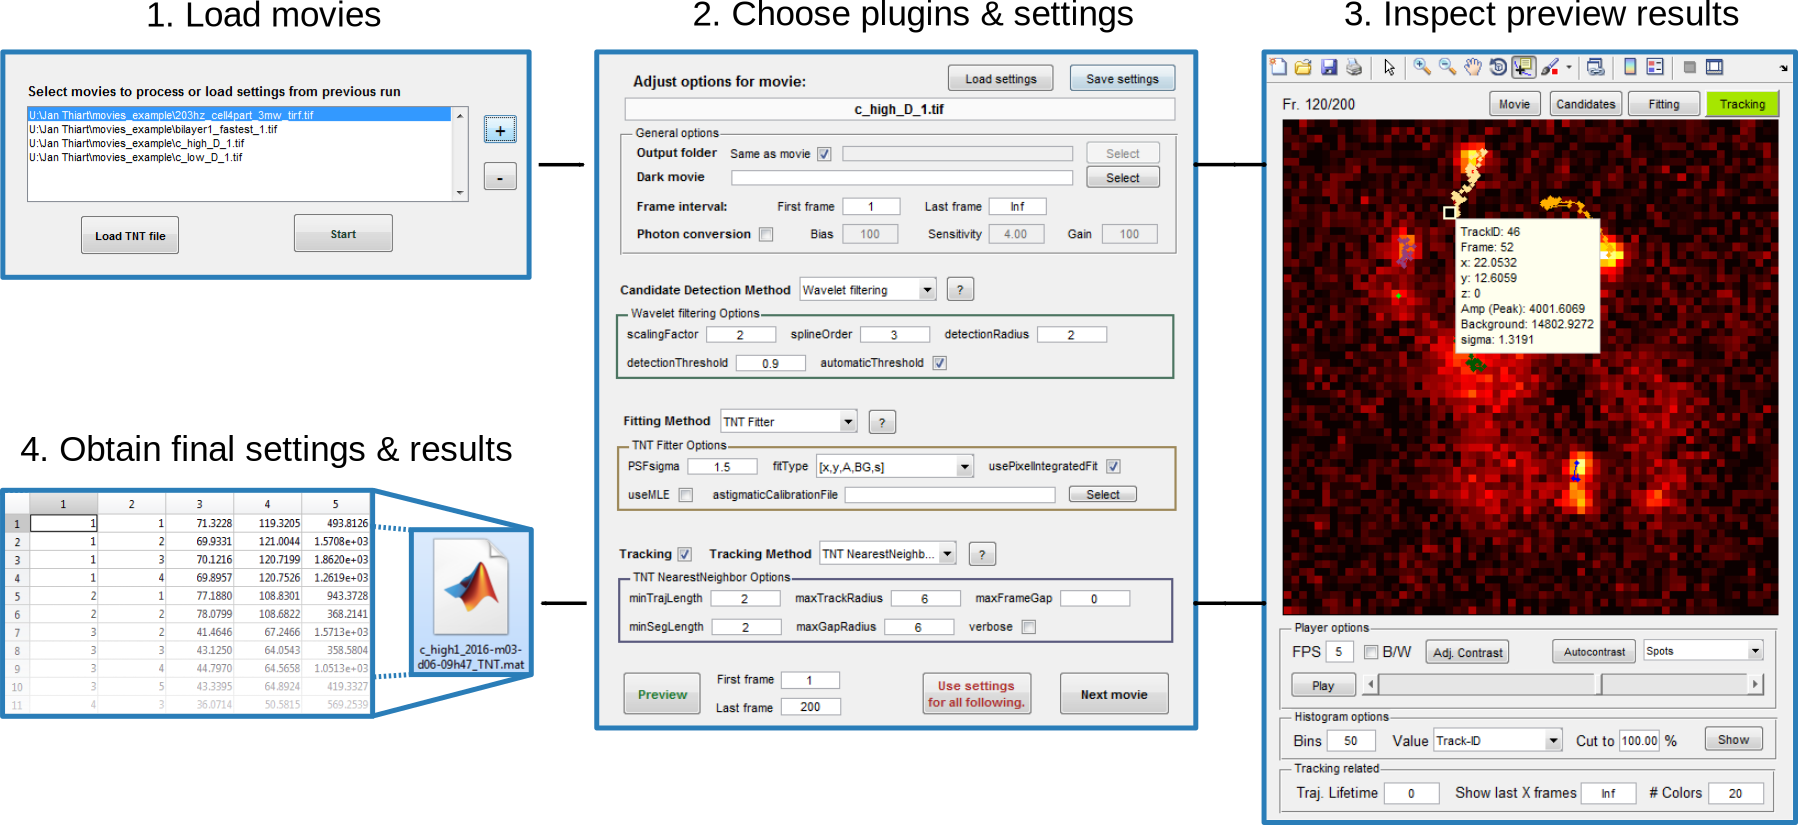
\includegraphics[width=0.9\textwidth]{./fig0.pdf} 
\caption{Program flow and user interface of TrackNTrace. First, a list of movies or a previously saved settings file is loaded before the main GUI is initialized. There, plugins for candidate detection, position refinement, and particle tracking are chosen and their settings adjusted for each movie. At any time during parameter tuning, a preview for an arbitrary part of the current movie can be computed and visualized. The visualizer is able to display the output from all stages (here shown in tracking mode). Selecting a candidate, localization, or track showcases the respective plugin-specific output (e.g. fitted parameter values). After parameter adjustment for all movies, the actual processing starts, saving each movie's output data along with the chosen settings in a single file.}
\label{fig:flowdiagram}
\end{figure}

\subsection{Startup (Fig. \ref{fig:flowdiagram}.1)}
When you first run \texttt{RunTrackNTrace.m}, the GUI as seen in figure~\ref{fig:flowdiagram}.1 pops up. Here, you can select the relevant movie files to process. Movies are added via the ``\textsf{+}'' button, where multiple movies can be selected in one go using the ``\textsf{Shift}'' key. Likewise, the ``\textsf{-}'' button removes the selected entry from the list. Pressing \textsf{Start} invokes the main GUI (fig. \ref{fig:flowdiagram}.2). If ``\textsf{Load TNT file}'' is pressed, a TrackNTrace settings file (MATLAB's \texttt{*.mat} file format, files end on \texttt{\textunderscore TNT}) can be selected, which loads all settings from a previous run, also starting the main GUI.

\subsection{Main GUI (Fig. \ref{fig:flowdiagram}.2)}
In the main GUI all processing settings are adjusted. On first startup it always shows the settings for the first movie in the list. The current settings can be saved to a file or previously saved settings loaded via the \textsf{Save Settings} and \textsf{Load settings} buttons on the top. Below the current file's name is displayed (hovering reveals full path). Next to the filename, a button opens the import options in case there are any (see section \ref{sec:importPlugin}). The main part of the GUI is designed for five processing steps:
\begin{enumerate}
 \item \textbf{Generating intensity image stack:} Measurements can be corrected for dark currents and camera artifacts. Algorithms based on quantitative analysis of photon signals (e.g. maximum-likelihood estimation, MLE) require subsequent conversion of analogue-digital-converter counts to photon numbers. If the import plugin supports TCSPC, a time gate can be defined.
 \item \textbf{Detecting candidates:} Potential sources of signal above the background noise are identified in each frame to obtain rough estimates of emitter positions with pixel precision. %This step is critical as misses or false detections cannot be distinguished from true events lateer.
  \item \textbf{Position refinement:} Each candidate's position estimate is refined with sub-pixel accuracy and additional information (background strength, brightness, dipole orientation, etc.) extracted. Commonly, this involves fitting a representation of the microscope's PSF to a subsection of the frame.
  \item \textbf{Tracking:} Positions separated in time are connected frame-by-frame to form trajectories. High particle density, intersecting tracks, and re-appearing, previously lost emitters are the main obstacles to overcome during this stage.
  \item \textbf{Post-processing:} Based on the tracks, additional properties can be determined. This step is used for lifetime fitting with the plugin \textsf{fitLT}.
\end{enumerate}

The first part corresponds to the \textsf{General options} panel, where the following elements can be adjusted:
\begin{itemize}[leftmargin=3.5cm]
\item[\textsf{Output folder}] Folder where the TNT output file is saved. The filename is always derived from the movies name with an additional timestamp and the ending \texttt{\textunderscore TNT}. For example: the output of a movie ``\texttt{data.tif}'' could become ``\texttt{data\textunderscore 2016-m03-d14-13h15\textunderscore TNT.mat}''. If \textsf{Same as movie} is checked, the output will be right next to the movie. Otherwise press \textsf{Select} to open a file dialogue where you can select a folder (or simply type one into the field directly). Leaving the field empty saves in the current MATLAB location.
\item[\textsf{Dark movie}] Select a movie (*.tif only) taken with the exact same camera settings used in your experiment but with the shutter closed. This movie is used to correct for non-isotropic camera sensitivity, dead pixels and other artifacts according to [1].
\item[\textsf{Frame interval}] Select the first and the last movie frame for processing. Anything not in this interval will be discarded. If \textsf{Last frame} is higher than the movie size or set to \textsf{Inf}, the whole movie is processed, starting at \textsf{First frame}. With \textsf{Binning} multiple subsequent frames are merged by summing their intensity.
\item[\textsf{Photon conversion}] If checked, the movie frames are converted from ADC counts to photons before they are handed to the plugins for processing. The conversion formula is
\begin{align}
I_{\texttt{phot}} = (I_{\texttt{ADC}}-\texttt{Bias})\times\texttt{Sensitivity}/\texttt{Gain}.
\end{align}
A conversion of this type is only meaningful for EMCCD cameras. The values for \texttt{Bias}, \texttt{Sensitivity} and \texttt{Gain} should be available in the camera's performance sheet. For TCSPC based import plugins \textsf{Photon conversion} is automatically activated with \texttt{Bias} 0, \texttt{Sensitivity} 1 and \texttt{Gain} 1.
\item[\textsf{Timegating}] If checked, only photons arriving between the time bins \textsf{Start} and \textsf{End} are used to generate the intensity movie. The button \textsf{Show TCSPC} generates a preview. Only available if the import plugin supports TCSPC.
\end{itemize}

The lower part houses the plugins for steps 2-5, where the plugin for each step is selected using a popup menu. The [ \textsf{?} ] button besides these menus shows an explanation of the currently selected plugin. Tracking (step 4) and post-processing (step 5) can optionally be disabled/enabled, the other two steps are always carried out. That said, the \texttt{Use candidate data} plugin for step 3 simply copies the data from step 2 and converts it to the right output format. As each plugin's inputs are different, we will not explain the plugins here, but rely on their explanation and their tooltip. \\

At the bottom left part of the GUI the preview button is placed, which starts the visualizer (see below) for the frame interval specified by   \textsf{First frame} and \textsf{Last frame} to the right of the button. This visualization is one of TrackNTrace's core features, making data analysis and parameter optimization much easier. The bottom right button either switches to the settings of the next movie in the list (displays ``\textsf{Next movie}) or starts processing all movies (displays ``\textsf{START processing}''). If all movies are alike, the ``\textsf{Use settings for all following}'' button applies the current movie's settings to all yet unadjusted movies in the list and starts the processing directly.\\[10pt]

\subsection{Preview/Visualizer (Fig. \ref{fig:flowdiagram}.3)}
The visualizer shows the data acquired from steps 2 through 5 (if available). Aside from its use by \texttt{RunTrackNTrace.m}, the visualizer can also be started directly by executing \texttt{TNTvisualizer.m} (check the file for the different input options). This is useful for viewing data from previous runs or any kind of movie that is supported by an import plugin. In the top right the type of data to display can be selected. If a data point is selected with the mouse, all corresponding output parameters from the plugin that computed it are shown. The counter in the top left shows the current/maximum frame. A panel with player options is below the movie. If results are loaded, additional options to analyze and display the data are available at the bottom of the player in a tabbed GUI. If a raw movie file is loaded frame interval, timegating and options provided by the import plugin are shown. Controls for panning/zooming and toggling of datatip, colorbar, legend and scalebar are located in the toolbar at the top of the window.

\paragraph{Player options}
\begin{itemize}[leftmargin=3cm]
\item[\textsf{FPS}] The frames per second (speed) the movie is played back with when \textsf{Play} is pressed.
\item[\textsf{FLIM}] If checked, the intensity is encoded as brightness (blend to black) and the lifetime according to the selected colormap.
\item[\textsf{invert}] If checked, the colormap is reversed.
\item[\textsf{Adj. contrast}] Shows a popup menu which allows manually changing the contrast.
\item[\textsf{Autocontrast}] The contrast is chosen automatically with a method chosen from the popup menu to the right. Similar to the popular \texttt{ImageJ} software, holding the \textsf{Shift} key during playback continously adjusts the contrast. 
	Currently included methods are: \\\hspace*{0.35cm}
	Spots: Emphasize highest 25\% intensity values.\\\hspace*{0.35cm}
	Min/Max: Contrast spans all values.\\\hspace*{0.35cm}
	98\% range: Cuts the lower and upper 1\% of intensities. 

\item[\textsf{$\gamma$}] Gamma correction of the intensities. $\gamma<1$ helps to enhance lifetime contrast in darker regions.
\item[\textsf{Colormap}] Drop-down menu with colormaps. The colormaps \textsf{heat}, \textsf{iso65}, \textsf{iso75} and \textsf{rainbow} are designed to be perceptionally uniform. The colormaps \textsf{iso65} and \textsf{iso75} are isoluminant. They are recommended for FLIM images to avoid cross-talk between lifetime and intensity.
\item[\textsf{Export}] Exports the current frame or movie according to the selected options. Press \textsf{Ctrl} and click to chose a frame range for stack export.
	Currently included options are: \\\hspace*{0.35cm}
	TIFF (Stack): exports the movie (including marker) as RGB TIFF stack.\\\hspace*{0.35cm}
	GIF (Stack): exports the movie (including marker) as GIF. Set FPS to control speed.\\\hspace*{0.35cm}
	TIFF (Frame): exports the current frame (including marker) as RGB TIFF.\\\hspace*{0.35cm}
	PNG (Frame): exports the current frame (including marker) as PNG.\\\hspace*{0.35cm}
	TIFF (Stack, int): exports the raw intensity movie.\\\hspace*{0.35cm}
	TIFF (Stack, tau): exports the raw lifetime movie.\\\hspace*{0.35cm}
	New figure: copies the current frame to a new figure.\\
	Please note that only TIFF (Stack, int) and TIFF (Stack, tau) preserve the original pixelsize.
\end{itemize} 

\paragraph{Histogram}
\begin{itemize}[leftmargin=3cm]
\item[\textsf{Value}] Parameter to histogram. What is available depends on the plugin that computed the current mode's data.
\item[\textsf{Bins}] Number of bins the histogram is computed for.
\item[\textsf{Cut to X \%}] Cuts (100-X)/2 \% of data from the lower and upper tails of the distribution before computing the histogram. 
\item[\textsf{All frames}] If checked, the data from all frames is used, otherwise from the current frame.
\item[\textsf{Avg tracks}] If checked, the selected value is average for each track before calculating histogram.
\item[\textsf{Gauss fit}] If checked, a Gaussian is fitted to the histogram.
\item[\textsf{Histogram}] Computes and displays the histogram of the selected value.
\item[\textsf{2\textsuperscript{nd} value}] Second parameter used for 2D and weighted histograms.
\item[2D Hist.] Computes and displays a 2D histogram of both selected values.
\item[Weighted Hist.] Computes and displays a histogram of the first selected value weighted by the second value.
\end{itemize}

\paragraph{Tracks (only affects \textsf{Tracking} mode)}
\begin{itemize}[leftmargin=3.5cm]
\item[\textsf{Traj. Lifetime}] Number of frames a trajectory is visible after its detection.
\item[\textsf{Show last X frames}] Shows only the past X frames of each trajectory.
\item[\textsf{\# Colors}] Number of colors the trajectories are displayed in. 
\end{itemize}

\paragraph{Filter}
\begin{itemize}[leftmargin=3cm]
	\item[\textsf{Expression}] Input field for a filtering expression. Standard Matlab syntax with support for vector operation, eg: \texttt{sigma<mean(sigma) \& Amp\_Peak\_>2*Background} 
	\item[\textsf{Value}] List of available filter parameters.
	\item[\textsf{Insert}] Inserts the currently selected value at the end of the filtering expression.
	\item[\textsf{Apply}] Applies the filtering expression to the current, filtered dataset. On success the expression turns red, on error red.
	\item[\textsf{Reset}] Resets the dataset of the current mode.
	\item[\textsf{Show table}] Opens a table with the dataset of the current mode. By default the filtered dataset is shown. \textsf{Ctrl} + Click opens the unfiltered dataset and colors rows filtered out dark.
	\item[\textsf{Export}] Exports the dataset of the current mode as \textsf{csv} or \textsf{xlsx}. By default the filtered dataset is used. \textsf{Ctrl} + Click exports the unfiltered one.
\end{itemize}

\paragraph{Reconstruct}
\begin{itemize}[leftmargin=3cm]
\item[\textsf{Method}] Method of reconstruction. Currently included are:
\begin{itemize}
\item[] Gaussian: Draws a pixel integrated, normalized Gaussian ($\sigma$=precision) at the position of each localization.
\item[] Weighted: 2D histogram of localization positions, each weighted with 1/precision.
\item[] Jitter: draws a point with a normal distributed random offset ($\sigma$=precision) for each localization. This is repeated $n$ (default: 5) times.
\item[] Points: 2D histogram of localization positions.
\end{itemize}
\item[\textsf{Create}] Performs the selected reconstruction and displays it in a new window.
\item[\textsf{Value}] Property used for the mean reconstruction.
\item[\textsf{Mean}] Reconstructs an image where the number of localization is given in the first channel and the local average of the selected value in a second channel. Use the \textsf{FLIM} option of the \textsf{TNTVisualizer} to view the second channel.
\item[\textsf{Pixelsize}] Pixelsize of the movie in nm.
\item[\textsf{SuperRes}] Ratio between the pixelsize in the reconstructed image and the original movie.
\item[\textsf{Loc. precision}] Localization precision in nm. For NaN the localization precision is estimated for each localization based on a modified Mortensen formula. (See [2])
\item[\textsf{Avg tracks}] If checked, position and selected value are averaged for each track before the reconstruction.
\end{itemize}

\paragraph{Drift}
\begin{itemize}[leftmargin=3cm]
\item[\textsf{Method}] Method for localization based drift correction. Currently included are:
\begin{itemize}
	\item[] RCC: redundant cross-correlation (see [3])
	\item[] DCC: direct cross-correlation (see [3])
	\item[] MCC: mean cross-correlation (see [3])
\end{itemize}
\item[\textsf{Calculate}] Calculates drift with the selected method based on the current, filtered dataset.
\item[\textsf{Export}] Exports the calculated drift as \textsf{csv} or \textsf{xlsx}.
\item[\textsf{Import}] Imports drift from a \textsf{csv} file. The file has to contain a header and the columns \textsf{x}, \textsf{y} and \textsf{frame}. If frames are missing the drift is interpolated.
\item[\textsf{Show}] Plots the calculated/imported drift and the currently applied drift in case it is different.
\item[\textsf{Apply}] Corrects the drift in the current dataset using the calculated/imported drift.
\item[\textsf{Resolution}] Resolution upscale of the intermediate images for drift correction. A higher resolution allows to detect smaller drift but requires more localization
\item[\textsf{$\Delta r$ max}] Error threshold for recalculating the drift in px. (Only used by RCC)
\item[\textsf{Seg. length}] Number of frames in each segment. A lower number increases the time resolution but reduces the localizations per segment and therefore the spatial resolution.
\item[\textsf{Reset}] Removes the drift correction from the current dataset.
\end{itemize}
\subsection{Headless mode}\label{sec:headless_mode}
TrackNTrace can also run without interactive user input. This headless mode is useful for batch processing of many files or systematic variation of options. For this \texttt{RunTrackNTrace} is called with input arguments as shown in the code example:
\begin{lstlisting}[style=Matlab-editor]
moviefiles = {'movie_1.tif','movie_2.tif','movie_3.tif'};
% This template can be genreated using "Save settings" in the settings GUI
tnttemplate = load('template_TNT.mat');
% If required, the plugin options can be manipulated.
tnttemplate.candidateOptions.PSFsigma = 1.5;
% Convert template to a cell array.
tntargs = [fieldnames(tnttemplate) struct2cell(tnttemplate)]';
% Run TrackNTrace: All files are processed with the same options
tntfiles = RunTrackNTrace(moviefiles,tntargs{:},...
   'showStartupGUI',false,... Disables the Startup GUI (file selection)
   'showSettingsGUI',false... Disables the Settings GUI
   );
\end{lstlisting}
\clearpage
\section{TrackNTrace output}\label{sec:datastructures}
All results obtained by TrackNTrace are saved in a \texttt{mat}-file in the format \texttt{'moviename\textunderscore timestamp\textunderscore TNT.mat'}. Here is a list of all variables it contains:
\begin{table}[!h]
\centering
\caption*{\textbf{TrackNTrace data structures}}
\label{tab:datastruct}
\begin{tabular}{p{.22\textwidth} p{.73\textwidth}}
\toprule
\multicolumn{1}{c}{Variable name} & \multicolumn{1}{c}{Description}\\ \midrule
\texttt{filename\textunderscore movie} & String containing full path of movie file. \\[5pt]
\texttt{metadata} & Struct returned by the import plugin containing information about the movie. \\[5pt]
\texttt{dark\textunderscore img} & 2D double array containing correction image to be added to each movie frame. \\[5pt]
\texttt{movieSize} & $1\times3$ matrix saving the size of the movie [rowPixel, colPixel, nrFrames] \\[5pt]
\texttt{firstFrame\textunderscore lastFrame} & $1\times2$ matrix [first frame, last frame] saving the first and last processed frame of the movie. This is important if only parts of a movie were read in and processed. \\[5pt]
\texttt{globalOptions} & Struct of general options variables set by the GUI. \\[5pt]
\texttt{candidateOptions} & Struct of candidate options parameters. Also contains the used plugins name and a parameter description for all output columns in \texttt{outParamDescription}. \\[5pt]
\texttt{refinementOptions} & Struct of refinement options parameters. Also contains the used plugins name and a parameter description for all output columns in \texttt{outParamDescription}. \\[5pt]
\texttt{trackingOptions} & Struct of tracking plugin parameters. Also contains the used plugins name and a parameter description for all output columns in \texttt{outParamDescription}. \\[5pt]
\texttt{postprocOptions} & Struct of post-processing plugin parameters. Also contains the used plugins name and a parameter description for all output columns in \texttt{outParamDescription}. \\[5pt]
\texttt{candidateData} & $n\times 1$ cell array of candidate positions where $n$ is the number of analyzed frames. Each cell contains a $k\times p$ double array, where $p$ is the number of model parameters and $k$ is the maximum amount of particles in the respective frame. Each row represents a unique candidate fit and the column order is $\mu_x$, $\mu_y$. These columns are mandatory for the refinement to work. Plugins can output extra data.\\
\texttt{refinementData} & $n\times 1$ cell array of refined positions where $n$ is the number of analyzed frames. Each cell contains a $k\times p$ double array, where $p$ is the number of model parameters and $k$ is the maximum amount of particles in the respective frame. Each row represents a unique fit and the column order according to the model PSF is $\mu_x$, $\mu_y$, $\mu_z$, $A$, $B$ (amplitude, background). These five columns are mandatory for most trackers to work correctly in step 4. Plugins can output extra data.\\
\texttt{trackingData} & 2D double array, list of trajectories with columns  [id,frame,$\mu_x$,$\mu_y$,$mu_z$] + additional columns. Every trajectory is given an id, starting at 1, after which the list is sorted. Frame number starts with 1.\\
\texttt{postprocData} & 2D double array, list of trajectories. Columns like \texttt{trackingData} + additional columns.\\
\bottomrule
\end{tabular}
\end{table}

\clearpage

\section{How to write a TrackNTrace plugin}\label{sec:howto_plugins}
This section explains how plugins are added to the TrackNTrace framework, with a concise demonstration of all features shown in \texttt{plugins/pluginDemo.m}. A plugin is defined as a function in a single file named ``\texttt{plugin\_NAME.m}'' inside the \texttt{plugins} subfolder of the TrackNTrace root directory. 

\subsection{Plugin header}
The function inside the file returns a \texttt{TNTplugin} object. In the simplest case, the file content looks like this:
\begin{lstlisting}[style=Matlab-editor]
function [plugin] = plugin_NAME()
name = 'Some candidate plugin';
type = 1; %1 for candidate, 2 for refinement, 3 for tracking, 
          %4 for post-processing, 5 for movie import
mainFunc = @arbitraryName_main;
outParamDescription = {'OutputVariableName1'; 'OutputVariableName2'};
plugin = TNTplugin(name, type, mainFunc, outParamDescription);
end

function [output] = arbitraryName_main(img, options, currentFrame) 
% Actual algorithm implemented here
end
\end{lstlisting}
While the four parameters used in the constructor are mandatory for every plugin, there are additional parameters that can be set optionally after the object is constructed. Here is a complete list:

\begin{longtable}[!h]{p{.235\textwidth} p{.71\textwidth}}
\caption*{\textbf{TNTplugin properties}}
\endfirsthead
\endhead
\toprule
\multicolumn{1}{c}{Property} & \multicolumn{1}{c}{Description}\\ \midrule
  \texttt{name} & Plugin name as displayed by the GUI. \\
  \texttt{type} & Integer, type of plugin. 1: Candidate detection, 2: Refinement, 3: Tracking, 4: Post-processing, 5: Import \\
  \texttt{mainFunc} & Handle to main function the plugin implementing the actual algorithm. For type 1 and 2 this is called by TrackNTrace in a loop for each individual frame of the input movie. The interface (output/input) of this function depends on the plugin type and must match the TrackNTrace specification (see below). \\
  \texttt{outParamDescription} &  Cell array of strings with description/name of all output parameters (columns) of the plugin \\
 \texttt{info} & Description of the plugin itself. Should describe the method and the general way how to use it. Supports \texttt{sprintf} modifiers directly (e.g. \texttt{\textbackslash n} for new line). \\
  \texttt{initFunc} &  Initialization function which is called once before the main is first executed. \\
  \texttt{postFunc} & Post-processing function which is called after the main function is last executed. \\
  \texttt{useParallelProcessing}&  Boolean. If false, TrackNTrace does not parallelize this plugins main function on a frame-by-frame basis for type 1/2 plugins. Useful if the main function itself is parallelized (e.g. a compiled multithreaded mex file) or if global information is needed (e.g. access to multiple frames of the movie).\\
  \bottomrule
\end{longtable}
\FloatBarrier

Parameters which can be adjusted by the GUI are defined by calling the \texttt{add\textunderscore param(par\textunderscore name, par\textunderscore type, par\textunderscore settings, par\textunderscore tooltip )} function of the newly created plugin instance. Let's look at the ``RadialSymmetry'' refinement plugin as an example:
\begin{lstlisting}[style=Matlab-editor]
function [plugin] = plugin_RadialSymmetry()
name = 'Radial symmetry';
type = 2;
mainFunc =  @refinePositions_radialSymmetry;
outParamDescription = {'x';'y';'z';'Amp (Peak)'; 'Background'; 'width'};

% Create the plugin
plugin = TNTplugin(name, type, mainFunc, outParamDescription);

% Description of plugin
plugin.info = ['Particle localization by radial symmetry centers. \n', ...
               'Algorithm published in Parthasarathy, NatMet 2012(9).'];
% Add parameters
plugin.add_param('PSFSigma',...
    'float',...
    {1.3,0,inf},...
    'PSF standard deviation in [pixel]. FWHM = 2*sqrt(2*log(2))*sigma.');
plugin.add_param('estimateWidth',...
    'bool',...
    true,...
    'Estimate particle width.');
end
\end{lstlisting}
 
As you can see, this plugin has two parameters of different types which will be visible in the GUI. Parameters are accessible for the plugin's main function via a struct (\texttt{candidateOptions}, \texttt{refinementOptions}, \texttt{trackingOptions}, \texttt{postprocOptions}) given as an input parameter. This means \texttt{PSFSigma} can be used inside the function as \texttt{options.PSFSigma}. Eventual whitespaces are replaced with underscores and dots within the parameter name are removed. Different parameters need different \texttt{par\textunderscore settings} as the third input. For example, the \texttt{bool} type parameter takes only the default value, while \texttt{float} type parameters need \texttt{\string{defaultValue, lowerBound, upperBound\string}}. The complete list of parameter types and needed settings is: 
\begin{table}[!h]
\centering
\begin{tabular}{p{0.135\textwidth} p{0.59\textwidth} p{0.185\textwidth}}
\toprule 
\multicolumn{1}{c}{\texttt{par\textunderscore type}} & \multicolumn{1}{c}{\texttt{par\textunderscore settings}} & \multicolumn{1}{c}{Example} \\ \midrule
  \texttt{\textquotesingle float\textquotesingle}  &Double variable, \texttt{\string{defaultValue, lowerBound, upperBound\string}} & \verb|{1.3,0,inf}| \\
   \texttt{\textquotesingle int\textquotesingle}    &Integer variable, \texttt{\string{defaultValue, lowerBound, upperBound\string}}& \verb|{4,-10,10}|\\
   \texttt{\textquotesingle bool\textquotesingle}   &Boolean variable, \texttt{defaultValue} & \texttt{true}\\
   \texttt{\textquotesingle string\textquotesingle} & String variable, \texttt{\textquotesingle defaultValue\textquotesingle} & \texttt{\textquotesingle @exp\textquotesingle} \\
   \texttt{\textquotesingle list\textquotesingle}  &  Interactive list box, \texttt{\string{\textquotesingle defaultEntry\textquotesingle, \textquotesingle Entry2\textquotesingle,...\string}}   & \texttt{\string{\textquotesingle x\textquotesingle,\textquotesingle [x,y]\textquotesingle\string}} \\
   \texttt{\textquotesingle filechooser\textquotesingle} & Interactive file chooser dialog \texttt{\string{\textquotesingle defaultDir\textquotesingle,\textquotesingle fileEnding\textquotesingle\string}} & \texttt{\string{\textquotesingle C:/Sci/\textquotesingle,\textquotesingle csv\textquotesingle\string}} \\
   \bottomrule
\end{tabular}
\end{table}
\FloatBarrier
The fourth parameter of the \texttt{add\textunderscore param} function is the tooltip shown when hovering over the parameter with the mouse (note: this supports \texttt{sprintf} modifiers, e.g. \texttt{\textbackslash{}n} for new line). \\

To  better structure the GUI users can call the \texttt{newRow()} function of a plugin instance between \texttt{add\textunderscore param(...)} calls which starts a new row in the graphical representation of the plugin. Furthermore, headings or descriptions can be added with \texttt{add\_text(text, horizontalAlignment, fontWeight, fontAngle, tooltip)}. The added text is automatically wrapped to fit into the plugin panel and always occupies its own rows (never shares rows with other parameters).   Possible values for \texttt{horizontalAlignment} are: 'left', 'center', 'right'.  Possible values for \texttt{fontWeight} are: 'normal', 'bold', 'light', 'demi'. Possible values for \texttt{fontAngle} are: 'normal', 'italic', 'oblique'.

\subsection{Plugin body}
A plugin must define a main function in \texttt{plugin.mainFunc}, which is called for every movie frame or only once in the case of tracking and post-processing. Unless explicitly forbidden, this process is parallelized using the parallelization toolbox. Movie import plugins have a slightly different syntax and are explained in section \ref{sec:importPlugin_syntax}.

The main functions have a different interface for every plugin type shown below:
\begin{lstlisting}[style=Matlab-editor]
% Type 1, candidate detection
function [candidates_frame_i] = mainFuncName(img, candidateOptions, i)
%Find candidates in 'i'-th frame 'img' of the processed frame interval using the options struct 'candidateOptions', and return a 2D position array candidates_frame_i with at least two columns for x and y position, one row per candidate
end
  
% Type 2, fitting/refinement
function [fits_frame_i]= mainFuncName(img, candidates_frame_i, refinementOptions, i)
%Refine candidate positions candidates_frame_i in 'i'-th frame 'img' of the processed frame interval using the options struct refinementOptions, and return a 2D position array fits_frame_i with at least five columns for x,y and z position, an intensity and a background value, one row per fitted candidate
end

% Type 3, tracking
function [trackingData] = mainFuncName(refinementData, trackingOptions);
        %OR
function [trackingData, trackingOptions] = mainFuncName(refinementData,trackingOptions);
%Track the positions in the cell array refinementData (cells of 2D arrays fits_frame) using the options struct trackingOptions and return a 2D array trackingData which should have at least the columns [track_id,frame,x,y,z]. Optionally also return trackingOptions
end

% Type 4, post-processing
function [postprocData] = mainFuncName(trackingData, postprocOptions);
%OR
function [postprocData, postprocOptions] = mainFuncName(trackingData, postprocOptions);
%Post-processes the tracks using the options struct postprocOptions and return a 2D array postprocData which should have at least the columns [track_id,frame,x,y,z]. Optionally also return postprocOptions.
end
\end{lstlisting}
Note that all variable names are arbitrary, however, their usage/order, their output structure, and their number has to match the above specifications. If your plugin cannot provide some output, e.g. a $z$-position or a background value, use 0 instead. 

If you already have a function \texttt{MyFunction.m} which, for example, finds candidates in an image and expects two parameters \texttt{p1} and \texttt{p2} which have been defined in the plugin header and saved in candidateOptions accordingly, adding the interface is very simple and could look like this:
\begin{lstlisting}[style=Matlab-editor]
function [candidate_xy] = wrapperForMyFunction(img, options, currentFrame)
candidates_xy = MyFunction(img,candidateOptions.p1,candidateOptions.p2);
end
\end{lstlisting}

\subsection{Optional pre- and post-processing functions}
The main functions are executed for every movie frame or all positions in the case of tracking. To avoid having to calculate derived parameters thousands of times althrough they are the same for all frames, or to perform post-processing steps which are only possible once the whole movie is processed, TrackNTrace can execute pre- and post-processing functions defined in \texttt{plugin.initFunc} and \texttt{plugin.postFunc}, if they are available. These functions are called just before or after the main function, respectively:
\begin{lstlisting}[style=Matlab-editor]
function [options] = initFuncName(options)

function [data, options] = postFuncName(data, options)
\end{lstlisting}
The \texttt{initFunc} can alter the \texttt{options} struct or add parameters to it before the main function is executed. This is useful for example for pre-computing masks for filter steps, creating lookup tables, or checking input parameter correctness. The \texttt{postFunc} function can be used to post-process \texttt{data} before it is saved and also add arbitrary information to \texttt{options}. Note that \texttt{data} (either \texttt{candidateData}, \texttt{refinementData}, \texttt{trackingData}, or \texttt{postprocData}) depends on the plugin type, see Sec.~\ref{sec:datastructures}). 

\subsection{Global variables and parallelization}
If needed, plugin functions can access external data not available to them via a function call by using global variables. Accessible variables are  \texttt{globalOptions}, \texttt{candidateOptions}, \texttt{refinementOptions}, \texttt{trackingOptions}, \texttt{movie}, \texttt{filename\textunderscore movie} and \texttt{imgCorrection} as defined in Sec.~\ref{sec:datastructures}. In addition the boolean \texttt{parallelProcessingAvailable} is true if parallel processing is available to TrackNTrace. They could be used as such:
\begin{lstlisting}[style=Matlab-editor]
function [output] = fittingFun(img, options, currentFrame)
global globalOptions;
img_in_photons = globalOptions.photonConversion;

if img_in_photons
   output = PhotonFun(img,options);
else
   output = NoPhotonFun(img,options);
end

end
\end{lstlisting}
For example, the \texttt{TNT NearestNeighbor} plugin uses global access to \texttt{refinementOptions} to copy the variable \texttt{outParamDescription} of all \texttt{refinementData} columns that are not needed for the tracking. 

Please note: The use of global variables inside type 1/2 plugin functions should be avoided, as functions with global variables can not be frame-by-frame parallelized by TNT, resulting in a possibly much slower execution time. Also note that, for memory reasons, the global \texttt{movie} variable gives access to the movie as returned from the import plugin (16-bit int without photon conversion for tif), regardless of the TrackNTrace settings. If your function both relies on having access to more than the current movie frame and needs a corrected and/or photon-converted movie, use the \texttt{correctMovie} function as in the following example:
\begin{lstlisting}[style=Matlab-editor]
global movie;
arbitaryMovieStack = movie{1}(:,:,1:4); % First 4 intensity frames
[correctedStack] = correctMovie(arbitraryMovieStack);
\end{lstlisting}

\subsection{File import plugins}\label{sec:importPlugin_syntax}
File import plugins are used as interface between TrackNTrace and the raw data. Any file-type specific processing should be done by the plugin. 
Import plugins are using the following fields.

\begin{longtable}[!h]{p{.235\textwidth} p{.71\textwidth}}
	\caption*{\textbf{TNTplugin properties for import plugins}}
	\endfirsthead
	\endhead
	\toprule
	\multicolumn{1}{c}{Property} & \multicolumn{1}{c}{Description}\\ \midrule
	\texttt{name} & Plugin name as displayed by the GUI. \\
	\texttt{type} & Integer, type of plugin. 5 for file import \\
	\texttt{mainFunc} & Handle to main function. (See syntax in code example below)\\
	\texttt{info} & Struct with information about the plugin. The fields \texttt{Description} and \texttt{supportedFormats} are mandatory. Possible fields are:
					\begin{itemize}[leftmargin=.2\textwidth,noitemsep,topsep=0pt]
						\item[\texttt{Description}] Description of plugin
						\item[\texttt{supportedFormats}] List of extensions, eg.: {\lstinline[style=Matlab-editor]|{{'*.tif;*.tiff','TIF'}}|}
						\item[\texttt{hasFLIM}] Boolean, {\lstinline[style=Matlab-editor]|true|} if the plugin can return FLIM images
						\item[\texttt{hasTCSPC}] Boolean, {\lstinline[style=Matlab-editor]|true|} if the plugin supports timegating and TCSPC extraction
						\item[\texttt{getTCSPC}] Function handle that returns the TCSPC of the first photons in the file. Syntax: 
						{\lstinline[style=Matlab-editor]|[tcspc,Resolution] = plugin.info.getTCSPC(file,maxPhotons)|}. Used for the preview of the timegating.
						\item[setFile] Function handle that is called once a new file is selected. Syntax: 
						{\lstinline[style=Matlab-editor]|valid = plugin.info.setFile(file)|}. Can return {\lstinline[style=Matlab-editor]|false|} to indicate incompatible files and/or set plugin options based on the file.
					\end{itemize}\nointerlineskip\\
	\texttt{postFunc} &  If \texttt{hasTCPSC} is \texttt{true}, this specifies an accumulation function to retrieve the TCSPC of the localisations.\\
	\texttt{initFunc} &  Optional function handle to generate cache for \texttt{plugin.postFunc}. \\
	\bottomrule
\end{longtable}
TrackNTrace always uses the first import plugin matching with the given file extension and not returning \texttt{false} on calling \texttt{plugin.info.setFile}.
See the implementation of \textsf{plugin\_loadPTU} and \textsf{plugin\_fitLT} for details on the syntax of \texttt{plugin.postFunc} and \texttt{plugin.initFunc}.

The movie is generated by TrackNTrace by calling \texttt{plugin.mainFunc} as in this example:
\begin{lstlisting}[style=Matlab-editor]
% Normal intensity movie:
FLIMflag = false; % plugins not supporting FLIM should ignore this input.
[movie,metadata] = plugin.mainFunc(importOptions,filename,...
                   [globalOptions.firstFrame, globalOptions.lastFrame],...
                   globalOptions.binFrame,FLIMflag);
% movie = {intensityMovie};

% FLIM movie with timegating
FLIMflag = true;
[movie,metadata] = plugin.mainFunc(importOptions,filename,...
                   [globalOptions.firstFrame, globalOptions.lastFrame],...
                   globalOptions.binFrame,FLIMflag,...
                   [globalOptions.tgStart globalOptions.tgEnd]);
% movie = {intensityMovie, lifetimeMovie};
\end{lstlisting}

The output \texttt{movie} should be a cell array containing the intensity movie as first element. The intensity movie is used for candidate detection and refinement should have the dimensions \texttt{[y,x,t]}. If not empty, the second cell is used by the \textsf{TNTVisualizer} in FLIM mode as lifetime movie. It should have the same dimensions as the intensity movie. Additional cells are ignored, but can be accessed by plugins using the global variable \texttt{movie}. The output \texttt{metadata} can be empty or a struct containing additional information about the movie. If present, the fields \texttt{pixelsize} and \texttt{pixelsize\_unit} are used by the \textsf{TNTVisualizer} for scalebar and reconstruction.

\FloatBarrier

\section{Provided TrackNTrace plugins (selection)}
Description of the input and output parameters of some of the provided plugins. All plugins provide a brief description and a explanation of their parameters in the tooltips.
\subsection{File import plugins}\label{sec:importPlugin}
\paragraph{TIFF (*.tif;*.tiff)}
Loads TIFF stacks. This plugin does not support color channels and provides no options.

\paragraph{PTU (PicoQuant Unified TTTR) single photon files (*.ptu)}
This plugin generates intensity and fluorescence lifetime movies for scanned measurements from the stream of photons saved in a PTU file. In a first step an intermediate index file is generated. During this step a shift between forward and reverse scans can be corrected automatically. The generated result can be cached along the raw data to save time when loading the same file again. This plugin supports timegating and TCSPC extraction.

This plugin provides following options:
\begin{itemize}[leftmargin=3cm]
\item[\textsf{alignBidirectional}] If enabled a shift from bidirectional scanning is corrected automatically by minimizing the difference between adjacent lines.
\item[\textsf{fastLT}] Method to estimate the lifetime for each pixel. Can be \textsf{std}, \textsf{mean} or \textsf{median}.
\item[\textsf{cacheMovie}] Number of versions to be cached. For 0 caching is disabled and the cache file deleted.
\end{itemize}

\subsection{Candidate detection plugins}

\paragraph{Cross correlation}
Candidate detection based on matching a Gaussian PSF template to the image using normalized cross-correlation. 

A Gaussian PSF template is created using the PSFsigma value provided by the user. The whole image is cross-correlated with this image using Matlab's \texttt{normxcorr2} function and maximums (meaning: emitters) in this correlation image are detected through non-maximum suppression by image dilation using the search window size \texttt{2*round(PSFsigma*distanceFactor)+1}. 
Candidates at the border of the image cannot be detected efficiently.

This plugin provides following options:
\begin{itemize}[leftmargin=3cm]
	\item[\textsf{PSFsigma}] Standard deviation of the PSF in pixels.\\
	\texttt{sigma = FWHM/(2*sqrt(2*log(2))) $\sim$ 0.21*lambda/NA} where \texttt{lambda} is the emission wavelength in pixels and \texttt{NA} is the numerical aperture of the objective.
	\item[\textsf{CorrThreshold}] Correlation threshold for pixels to count as emitter candidates. \\
	Must be between 0 and 1, a good range is 0.25 (many low quality candidates) to 0.4 (fewer, higher quality candidates).
	\item[\textsf{distanceFactor}]The local maximum search window size is \texttt{2*round(PSFsigma*distanceFactor)+1}. \\
	Lowering this value let's you detect candidates closer to each other but lowers candidate quality.
\end{itemize}

\paragraph{Wavelet filtering}
Candidate detection based on wavelet filtering with B-splines.

The algorithm performs a wavelet decomposition of the original image up to wavelet level 2. The result is an image where low-frequency components (i.e. emitters) of a shape and intensity distribution close to the B-spline kernel are highly elevated against high-frequency components such as noise. Maximums in the filtered image are then detected through local maximum suppression by image dilation. See Izeddin et al, Opt. Express 20(3),2012, doi: 10.1364/OE.20.002081 for details.

This plugin provides following options:
\begin{itemize}[leftmargin=3cm]
\item[\textsf{scalingFactor}] Wavelet scaling factor. This determines how fast the B-spline filter kernel falls of at the edges. Lower = greater falloff, which means sharper, more insular features. Values lower than 2 tend to find single pixels as candidates which is not recommended.
\item[\textsf{splineOrder}] B-spline order. Determines how smooth the filter falls off towards the edge. Higher = smoother falloff which correspond to larger, ``flatter" structures.
\item[\textsf{detectionRadius}] Size of local maximum detection window. Should be roughly similar to B-spline order.
\item[\textsf{detectionThreshold}] Detection threshold. Higher means less detected candidates.
\item[\textsf{automaticThreshold}] If set to true, the standard deviation of the wavelet filtered image at wavelet level 1 times the \texttt{detectionThreshold} is taken as the absolute peak intensity threshold. In this case, setting \texttt{detectionThreshold} from 0.8 to 1.2 is recommended. Otherwise, \texttt{detectionThreshold} is directly compared against the wavelet image in which case values between 3 and 5 usually provide usable results.
\end{itemize}
\paragraph{Import CSV}
This plugin imports a list of localizations from a CSV file, eg. as exported from ThunderSTORM. Ensure that x, y and potentially sigma are in the unit pixels and the frame range matches that of the movie. To pass the data without modification to the tracking plugin, use the refinement plugin \textsf{Use candidate data}. Without the options \textsf{sigma} and \textsf{otherValues} only x and y are imported, as required for the TNT Fitter.

This plugin provides following options:
\begin{itemize}[leftmargin=3cm]
	\item[\textsf{CSVfile}] Select a CSV file to import.
	\item[\textsf{sigma}] If checked, the sigma of the PSF is imported
	\item[\textsf{otherValues}] If checked, all additional columns present in the CSV are imported.
\end{itemize}
\subsection{Refinement plugins}
\paragraph{TNT Fitter}
Refine candidate positions by fitting a Gaussian PSF to candidate positions in C++.

The fitting code utilizes the ceres-solver library for optimization currently developed by Google (2015).

This plugin provides following options:
\begin{itemize}[leftmargin=3cm]
	\item[\textsf{PSFsigma}] Standard deviation of the PSF in pixels.\\	
		\texttt{sigma = FWHM/(2*sqrt(2*log(2))) $\sim$ 0.21*lambda/NA} where \texttt{lambda} is the emission wavelength in pixels and \texttt{NA} is the numerical aperture of the objective.
	\item[\textsf{fitType}] Fit positions (xy), amplitude \& background (A,BG), sigma (s, or sx \& sy for elliptic Gaussian), and angle (for a rotated elliptic Gaussian).
	\item[\textsf{usePixelIntegratedFit}] Use a pixel integrated Gaussian PSF for fitting which emulates the discrete pixel grid of a camera chip. This is automatically disabled when fitting a rotated Gaussian.
	\item[\textsf{useMLE}] Use Maximum Likelihood Estimation in addition to Least-squares optimization. MLE fitting absolute requires photon conversion!
	\item[\textsf{astigmaticCalibrationFile}] For astigmatic imaging, please select a calibration file created with  the \textsf{TNT z-calibration} plugin. Leave empty otherwise!
\end{itemize}
\subsection{Tracking plugins}
\paragraph{TNT NearestNeighbor}
Track particles using simple and fast nearest neighbor tracking with gap-closing implemented in C++

Implementation uses the nanoflann library written by Marius Muja, David G. Lowe and Jose Luis Blanco. Nanoflann is under the BSD license.

This plugin provides following options:
\begin{itemize}[leftmargin=3cm]
	\item[\textsf{minTrajLength}] Minimum length of trajectories in [frames].
	\item[\textsf{maxTrackRadius}] Maximum allowed linking distance between two localizations in [pixels].
	\item[\textsf{maxFrameGap}] Maximum allowed time gap between two segments used for gap closing in [frames]. When fluorophores blink or disappear, they obviuosly cannot be tracked anymore. If they reappear, however, tracked segments can be stitched back together. 0 = no gap closing.
	\item[\textsf{minSegLength}] Minimum length of trajectory segments BEFORE gap closing in [frames].
	\item[\textsf{maxGapRadius}] Maximum allowed linking distance between two segments uses for gap closing in [pixels].
	\item[\textsf{outputLength}] Adds the number of localizations to each track
	\item[\textsf{verbose}] Switch on to see tracking progress in command window.
\end{itemize}
\subsection{Post-processing plugins}
\paragraph{fitLT}
This plugin extracts the TCSPC from a definable area around each localization or track and determines the corresponding lifetime. It requires an import plugin that supports TCSPC extraction.

This plugin provides following options:
\begin{itemize}[leftmargin=3cm]
	\item[\textsf{position}] Controls how the position of each tracks is processed. options are:
	\begin{itemize}[leftmargin=2cm]
		\item[\textsf{preserve}] uses the positions provided.
		\item[\textsf{average}] averages the position over the length of the track.
		\item[\textsf{refit}] performs a Gaussian MLE fit on an sum image of all frames of the track.
	\end{itemize}
	\item[\textsf{maskRadius}] Radius of the mask for the TCSPC extraction in units of $\sigma_\mathrm{PSF}$. For each frame, a constant mask size is used which based on the median $\sigma_\mathrm{PSF}$ in that frame.
	\item[\textsf{sumTCSPC}] If enabled, the TCSPCs of all localization within one track are summed.
	\item[\textsf{exportTCSPC}] If enabled, the TCSPCs are saved in the struct postprocOptions.
	\item[\textsf{fitType}] Method for lifetime determination:
	\begin{itemize}[leftmargin=2cm]
		\item[\textsf{fast lifetime}] estimates the lifetime using the std of the arrival times. (Very fast)
		\item[\textsf{monoexponential MLE}] performs an monoexponential MLE tailfit with a Nelder-Mead simplex search.  Uses \textsf{average DistFit} to generate an initial guess. (Most accurate for monoexponential data)
		\item[\textsf{average DistFit}] generates 10 lifetime decays logarithmically spaced between \textsf{minLT} and \textsf{maxLT}, finds their amplitudes by a non-negative least-square optimization and returns the amplitude weighted lifetime average.
		\item[\textsf{maximum correlation}] generates 500 lifetime decays logarithmically spaced between \textsf{minLT} and \textsf{maxLT}, calculates their correlation with the TCSPC and returns the lifetime with highest correlation.
	\end{itemize}
\item[\textsf{cutoff}] cutoff for tail fits with respect to the maximum of the TCSPC.
\item[\textsf{minAmp}] minimum number of photons in the TCSPC to perform a fit. Low number of photon TCSPCs are slower to fit and the results are less certain.
\item[\textsf{minLT}] lower bound for lifetime fitting.
\item[\textsf{maxLT}] upper bound for lifetime fitting.
\item[\textsf{attempts}] number of fit attempts. For each attempt the initial lifetime is slightly varied. (only used by \textsf{monoexponential MLE})
\item[\textsf{tolerance}]relative termination tolerance of the fitting. (only used by \textsf{monoexponential MLE})
\end{itemize}

The plugin adds (depending on the options) following columns to the output:
\begin{itemize}[leftmargin=3cm]
	\item[\textsf{tau-fast}] standard deviation of the photon arrival times. (Equivalent to \textsf{fitType} = \textsf{fast lifetime})
	\item[\textsf{nphoton}] number of photons in the TCSPC.
	\item[\textsf{lt-tau}] lifetime determined with the selected \textsf{fitType}.
	\item[\textsf{lt-amp}] amplitude of the fit in total photons. (only for \textsf{monoexponential MLE} and \textsf{average DistFit})
	\item[\textsf{lt-bg}] background of the fit in total photons. (only for \textsf{monoexponential MLE} and \textsf{average DistFit})
	\item[\textsf{lt-chi2}] reduced $\chi^2$ of the fit (only for \textsf{monoexponential MLE} and \textsf{average DistFit})
	\item[\textsf{lt-corr}] correlation between \textsf{lt-tau} and the TCSPC  (only for \textsf{maximum correlation})
\end{itemize}
\clearpage

\section{References}
\begin{itemize}
\item [{[1]}]  Hirsch M, Wareham RJ, Martin-Fernandez ML, Hobson MP, Rolfe DJ: A Stochastic Model for Electron Multiplication Charge-Coupled Devices {--} From Theory to Practice. PLoS ONE 8(1), 2012.
\item[{[2]}] Rieger B, Stallinga S: The lateral and axial localization uncertainty in super-resolution light microscopy. ChemPhysChem, 15(4), 2014.
\item[{[3]}] Wang Y, Schnitzbauer J, Hu Z, Li X, Cheng Y, Huang Z-L, Huang B: Localization events-based sample drift correction for localization microscopy with redundant cross-correlation algorithm. Optics Express, 22(13), 2014.
\end{itemize}

\end{document}

\item [{[2]}] Mortensen, KI, Churchman SL, Spudich, JA, Flyvbjerg H: Optimized localization analysis for single-molecule tracking and super-resolution microscopy. Nature Methods 7, 377 {--} 381, 2010.
\item [{[3]}] Jaqaman K et al: Robust single-particle tracking in live-cell time-lapse sequences. Nature Methods 5, 695 {--} 702, 2008.

\section{How TrackNTrace works}\label{sec:in-depth}
After storing all options, reading in the movie and, if applicable, a closed shutter movie for correction, the fitting routine starts. First, the movie frame is cleaned up by adding a correction image obtained from the closed shutter movie as described in [1] and then converted to a photon count image if possible. Then, the respective candidate search function is called for the respective frame and the result is passed to the fit function. Depending on the settings, candidate search is carried out in each frame or only once for the first (or last) frame or an average image of the first few (or last few) frames. In the latter case, fit results from the frame before are passed to the fit function in the next iteration. \\
Two candidate search mechanism are possible: Normalized cross-correlation and intensity filtering. For cross-correlation, a Gaussian PSF mask is created and the \texttt{normxcorr2} function is called to calculate a correlation image of the original movie frame. This image is then processed with a local maximum filter using \texttt{imdilate}. Pixels with a correlation value higher than the user-provided threshold are accepted as spot candidates. In the intensity filtering step, the image is convolved with a normalized filter kernel  consisting of a moving average window and a Gaussian bell curve of $\sigma = \unit{1}{\mathrm{px}}$ against discretization noise before being processed with a local maximum filter. The kernel has a window size of $w = 2r+1$ where $r$ is the spot radius given by the user. Next, a local background image [4] is calculated and all pixels have to pass two tests: The intensity must be among the top $q\%$ in the image and $1-\mathrm{CDF}(\mu_b,\sigma_b) \leq p$ must hold, where CDF ist the normal distribution cumulative density function, and $\mu_b$ and $\sigma_b$ are mean and standard deviation of the local background. $p$ and $q$ are user-provided thresholds.\\[10pt]
A list of spot candidate positions is passed to a \texttt{Mex} file which handles all fitting procedures. First, a square quadrant $I_\mathrm{exp}$ around a candidate pixel is fit to a 2D Gaussian,
\begin{align*}
I_\mathrm{theo}(x,y) = A\exp\left(-\frac{(x-\mu_x)^2}{2\sigma^2} - \frac{(y-\mu_y)^2}{2\sigma^2}\right) + B \quad\mathrm{with}\quad \min_\theta \sum_x\sum_y \left(I_\mathrm{theo}-I_\mathrm{exp}\right)^2
\end{align*}
where $\theta = (A,\mu_x,\mu_y,B,\sigma)$. Fitting $\sigma$ can be disabled by the user. A more accurate model can be obtained by taking into account the finite size of the camera chip pixel grid, where all signal photons hitting any point within a square pixel are accumulated:
\begin{align*}
I_\mathrm{theo, px} &= \int\limits^{+1\slash 2}_{-1\slash 2} \D x \int\limits^{+1\slash 2}_{-1\slash 2} \D y\: I_\mathrm{theo} \\
&= \frac{A \pi \sigma^2}{2}\cdot \left[\mathrm{erfc}\,\left(-\frac{x-\mu_x+1\slash 2}{\sqrt{2} \sigma}\right) - \mathrm{erfc}\,\left(-\frac{x-\mu_x-1\slash 2}{\sqrt{2} \sigma}\right)\right] \times \\
&\quad \left[\mathrm{erfc}\,\left(-\frac{y-\mu_y+1\slash 2}{\sqrt{2} \sigma}\right) - \mathrm{erfc}\,\left(-\frac{y-\mu_y-1\slash 2}{\sqrt{2} \sigma}\right)\right] +B
\end{align*}
Here, $\mathrm{erfc}$ is the complementary error function. Note that $x$- and $y$- dimension are decoupled, meaning that the two terms only have to be calculated once for one column and one line. Residual minimization is done by a Least-squares Levenberg-Marquardt algorithm. The result can be fitted again using Maximum Likelihood Estimation which is proven to yield the best possible result [2]:
\begin{align*}
\min_\theta (-\log\mathcal{L}) = \min_\theta (I_\mathrm{theo}(\theta) - I_\mathrm{exp} \ln I_\mathrm{theo}(\theta))
\end{align*}
All optimization steps rely on the \texttt{ceres-solver} library, an open-source optimization library written in \CC by Google Inc. We chose ceres for its very high performance, great customizability and the possibility of calculating all necessary first-order derivatives by using automatic differentiation which does not require user input and is therefore more robust. The MATLAB implementation by Simon Christoph Stein is available on the MATLAB file exchange where you can also find all necessary files and instructions for building {TrackNTrace}:  \href{http://www.mathworks.com/matlabcentral/fileexchange/52417-fast-gaussian-point-spread-function-fitting--mex-}{http://www.mathworks.com/matlabcentral/fileexchange/52417-fast-gaussian-point-spread-function-fitting--mex-}\\[10pt]
% FIXME \url did not break the url properly, even after trying different options/packages for 20 minutes.. (latex, *rolleyes*)
 After fitting is finished and if tracking is enabled, the result array is converted to a format suitable for the chosen tracker and passed to the tracking routine. Currently there are two options available: u-Track [3], and a custom, highly efficient nearest-neighbor tracker written in \CC. Depending on the tracker, the time complexity of particle linking is at least quadratic in the number of particles, linear in the number of frames and quadratic or even exponential in the number of gap frames. In u-Track's case, splitting the movie into several parts can be much faster than processing all positions in a single batch. In such situations, particles within and directly after such a border or split frame are tracked again to try to re-link trajectory segments artificially cut in half by splitting the movie. Gap frames cannot be accounted for in this case, therefore, caution is advised when using larger gap values and splitting numbers together.\\
For every tracker, the end result is an array containing all trajectories with recorded frame number, and respective $xy$- position and amplitude. Every trajectory has a unique id to facilitate post-processing. \\
While all tracking algorithms are handled more or less the same, u-Track is an exception. u-Track can handle very difficult scenarios such as Brownian-directional motion-switching, particle merging and splitting and provides a large number of user-input variables for this. These options are all hidden in the \texttt{parseUtrackOptions.m} file and are only meant to be changed by an experienced user. Caution is advised.

\clearpage















































